\documentclass[10pt,aspectratio=169]{beamer}

\usetheme[numbering=fraction,progressbar=none]{metropolis}
\usepackage{booktabs}
\usepackage{array}
\usepackage{tikz}
\usepackage{graphicx}
\usefonttheme{default}

\definecolor{RailwayBlue}{HTML}{1F3864}
\definecolor{DismissalRed}{HTML}{C0392B}
\setbeamercolor{normal text}{fg=black,bg=white}
\setbeamercolor{structure}{fg=RailwayBlue}
\setbeamercolor{frametitle}{fg=white,bg=RailwayBlue}
\setbeamercolor{title}{fg=RailwayBlue}
\setbeamercolor{subtitle}{fg=RailwayBlue}
\setbeamercolor{progress bar}{fg=RailwayBlue,bg=RailwayBlue!20}
\setbeamercolor{alerted text}{fg=RailwayBlue}
\setbeamertemplate{navigation symbols}{}
\setbeamertemplate{frame numbering}{fraction}
\setbeamertemplate{footline}{%
  \begin{beamercolorbox}[wd=\paperwidth,ht=2.5ex,dp=1.5ex,rightskip=1.5em]{page number in head/foot}%
    \usebeamerfont{page number in head/foot}\insertframenumber/\inserttotalframenumber
  \end{beamercolorbox}%
}

\title{Union Threat and Promotion Practices in Victorian Railways}
\subtitle{Preliminary Evidence from LNWR Birmingham, 1875--1924}
\author{Keitaro Ninomiya}
\institute{University of Illinois at Urbana-Champaign}
\date{May 2026}

\begin{document}

\begin{frame}{Research Question}
\begin{itemize}
  \item The 1875 Amalgamated Society of Railway Servants (ASRS) established branch networks across England
  \item Did proximity to union branches cause railway management to alter promotion practices?
  \item Two competing channels:
    \begin{enumerate}
      \item \textbf{Management response:} Union threat slows promotion as discipline/deterrence
      \item \textbf{Composition:} ASRS collapse (1880--82) changed workforce composition via dismissals
    \end{enumerate}
  \item Identification: pre-1875 accident rates instrument for union branch location
\end{itemize}
\end{frame}

\begin{frame}{Data Sources}
\small
\begin{tabular}{p{0.27\textwidth}p{0.27\textwidth}p{0.18\textwidth}p{0.22\textwidth}}
\toprule
\textbf{Source} & \textbf{Coverage} & \textbf{N} & \textbf{Key Variables} \\
\midrule
ASRS Balance Sheets 1875 & Nationwide & 6,066 members; 139 branches & Name, occupation, join date, branch location \\
\addlinespace
Railway Personnel Registers (Ancestry/TNA) & LNWR Birmingham; GWR Birmingham; GWR Aylesbury & 2,257 workers & Name, entry year, grade, promotion dates, station transfers \\
\addlinespace
Accident Records (Board of Trade) & England, pre-1875 & 778 incidents & Location (lat/lon), cause, fatalities, injuries \\
\bottomrule
\end{tabular}

\vfill
\footnotesize Proof of concept at LNWR Birmingham. Sheffield Midland register (1833--1888) download pending.
\end{frame}

\begin{frame}{The Rise and Fall of the ASRS}
\begin{itemize}
  \item \textbf{1871:} ASRS founded with support of Liberal MP Michael Bass
  \item \textbf{1872:} Peak membership of 17,247 --- tiny fraction of 250,000 railway workers
  \item \textbf{1875:} Annual balance sheets record 139 branches nationwide; concerns over member fatalities drive organising
  \item \textbf{1879:} GWR dismisses petitioning members; companies increase working week to 66 hours
  \item \textbf{1880:} ASLEF founded --- engine drivers and firemen split from ASRS
  \item \textbf{1882:} ASRS membership collapsed to 6,321
  \item \textbf{1913:} ASRS merges into National Union of Railwaymen
\end{itemize}

\end{frame}

\begin{frame}[plain]
\begin{center}
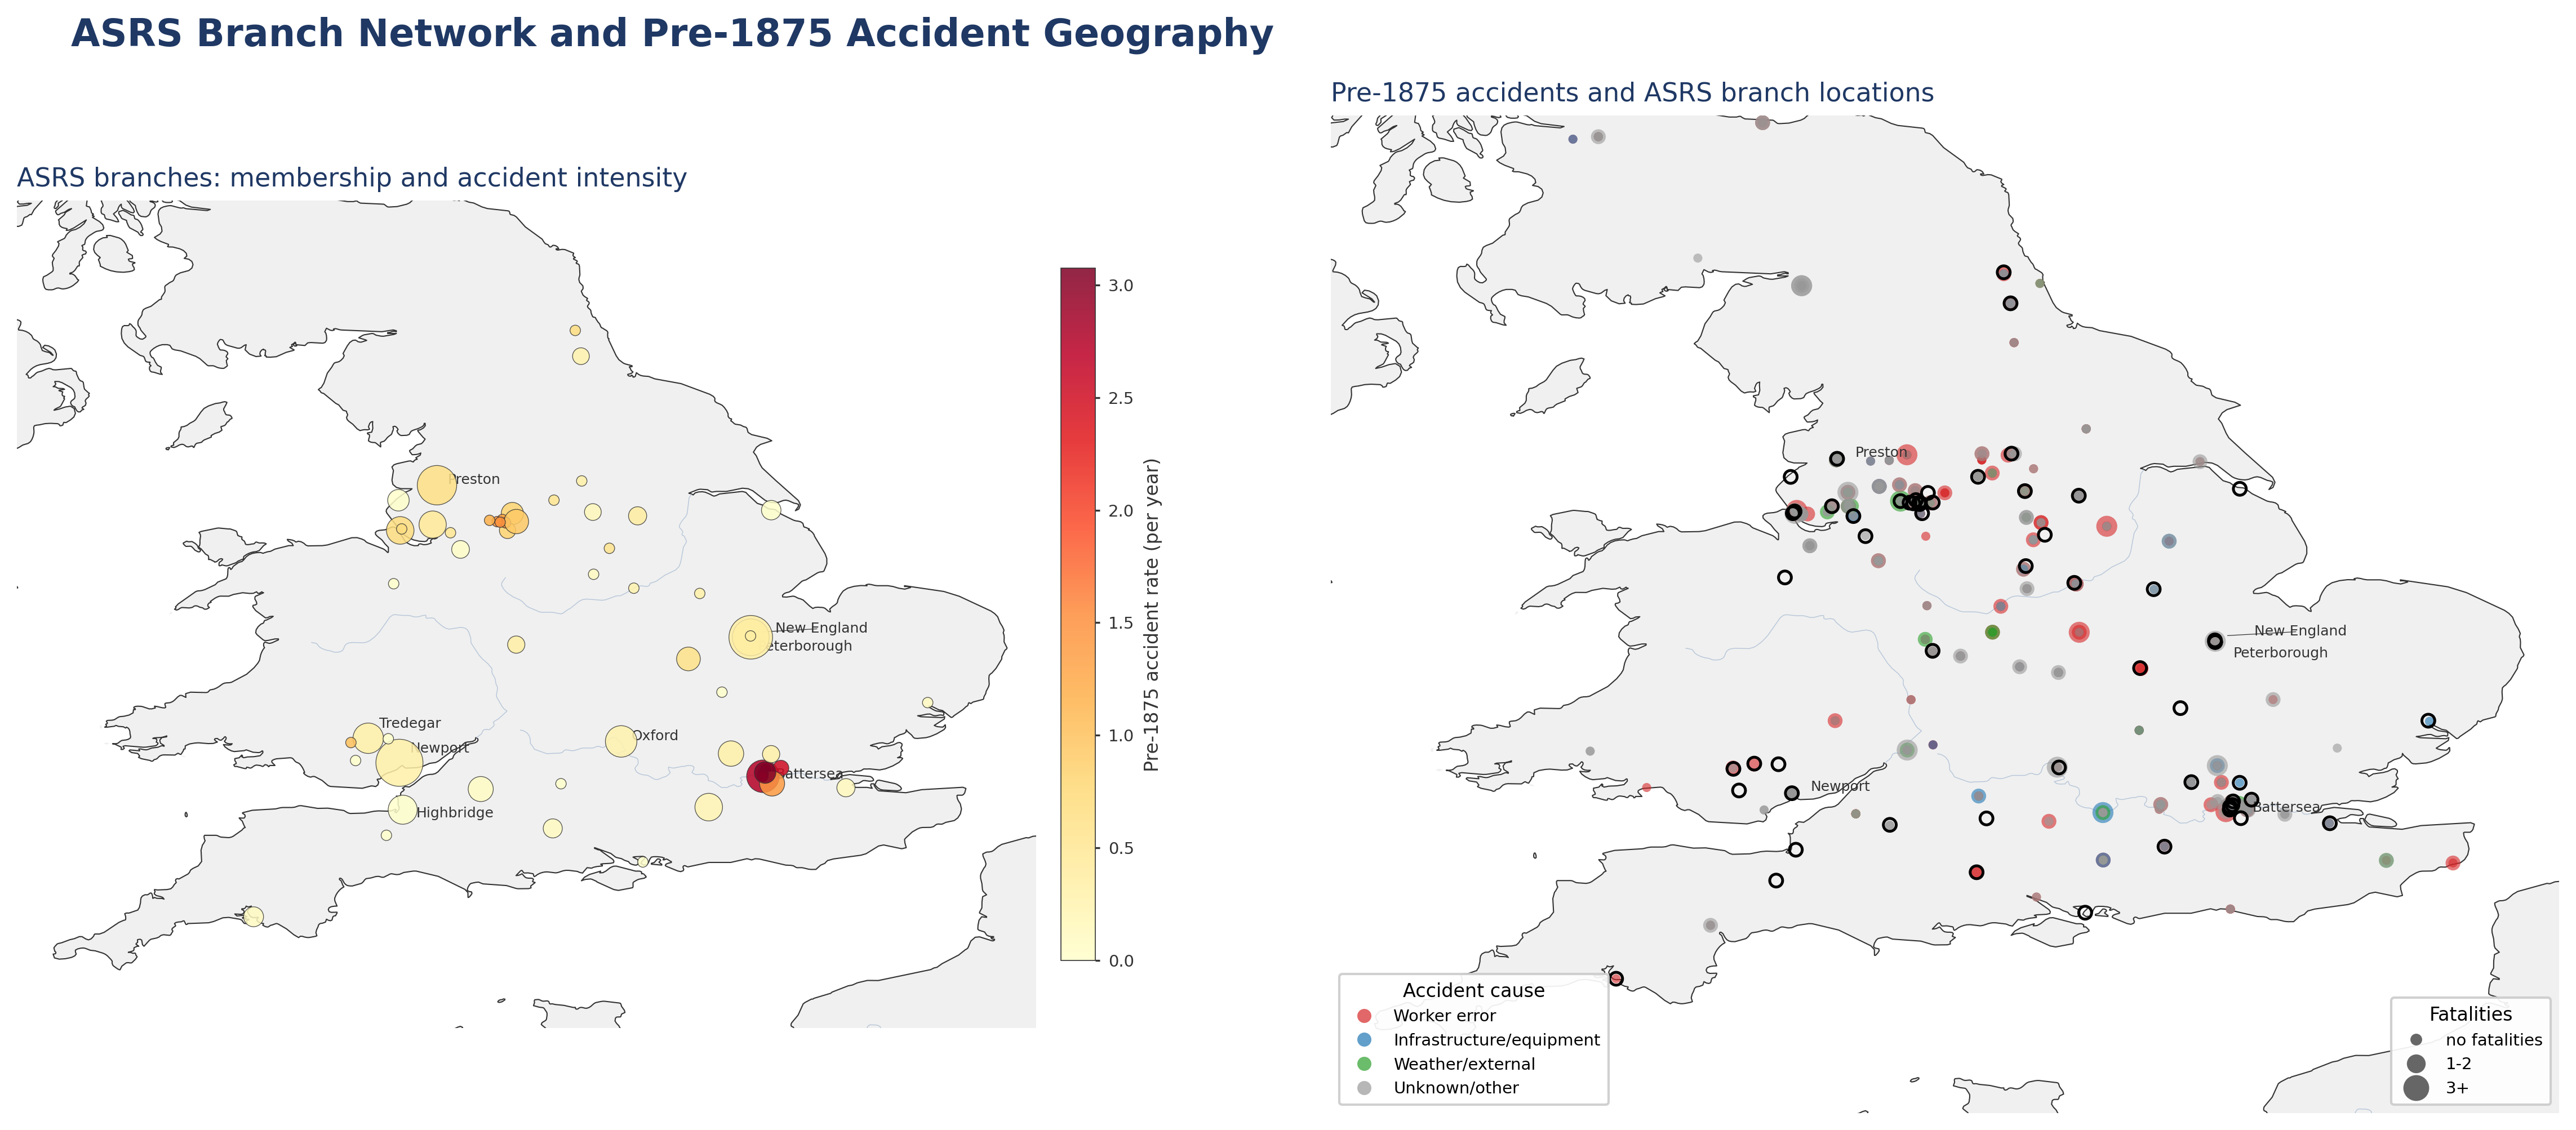
\includegraphics[width=\textwidth]{../combined_map.png}
\end{center}
\end{frame}

\begin{frame}{Accident Location Predicts Union Branch Location}
\centering
\footnotesize
\[
\mathbf{1}\{\text{ASRS branch in RD}_r\}
= \alpha + \beta\,\mathbf{1}\{\text{pre-1875 accident in RD}_r\}
+ X_r'\gamma + \delta_g + \varepsilon_r
\]

\vspace{-0.15cm}
\scriptsize
\begin{tabular}{lcccc}
\toprule
 & (1) Pooled & (2) County FE & (3) Division FE & (4) Line FE \\
\midrule
Has accident & 0.829$^{***}$ & 0.830$^{***}$ & 0.829$^{***}$ & 0.832$^{***}$ \\
 & (0.038) & (0.039) & (0.038) & (0.047) \\
\midrule
Observations & 514 & 511 & 514 & 388 \\
\(R^2\) & 0.780 & 0.754 & 0.764 & 0.776 \\
Fixed effects & None & County & Division & Railway line \\
\bottomrule
\end{tabular}

\vspace{0.35cm}
\begin{minipage}{0.88\textwidth}
\footnotesize
Unit of observation is the 1851 Registration District with at least one rail station in England and Wales.
Dependent variable equals one if the district has at least one ASRS branch.
Key regressor equals one if the district has a pre-1875 railway accident.
All columns control for log(area+1) and log(stations+1). HC1 robust standard errors in parentheses.
\end{minipage}
\end{frame}

\begin{frame}{LNWR Birmingham: Proof of Concept}
\begin{columns}[T,onlytextwidth]
\column{0.50\textwidth}
\textbf{\color{RailwayBlue}Register Description}
\begin{itemize}
  \item Birmingham Central District Guards Register
  \item RAIL 410, Piece 0246 (TNA/Ancestry)
  \item Coverage: 1879--1924
  \item 423 workers with valid entry year
  \item Nearest ASRS branch: Dudley (13km)
  \item Format A: explicit grade progression dates recorded
\end{itemize}

\column{0.44\textwidth}
\textbf{\color{RailwayBlue}Grade Progression}
\vspace{0.15cm}

\small
\begin{tabular}{ll}
\toprule
\textbf{Grade} & \textbf{Description} \\
\midrule
Pit Goods Guard & Entry grade \\
Shunter & Intermediate \\
Goods Guard & Full promotion \\
\bottomrule
\end{tabular}

\vspace{0.45cm}
\footnotesize Promotion = attaining Goods Guard or Shunter grade
\end{columns}
\end{frame}

\begin{frame}{Promotion and Dismissal Rates by Entry Cohort}
\begin{minipage}[t]{0.48\textwidth}
\centering
\textbf{Promotion Rate}

\vspace{0.12cm}
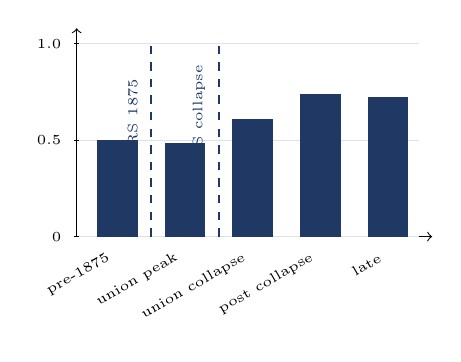
\begin{tikzpicture}[x=0.86cm,y=2.45cm]
  \draw[->] (0,0) -- (5.25,0);
  \draw[->] (0,0) -- (0,1.08);
  \foreach \y/\label in {0/0,0.5/0.5,1.0/1.0} {
    \draw[RailwayBlue!15] (0,\y) -- (5.05,\y);
    \draw (-0.04,\y) -- (0.04,\y) node[left=3pt] {\tiny \label};
  }
  \fill[RailwayBlue] (0.30,0) rectangle (0.90,0.500);
  \fill[RailwayBlue] (1.30,0) rectangle (1.90,0.486);
  \fill[RailwayBlue] (2.30,0) rectangle (2.90,0.609);
  \fill[RailwayBlue] (3.30,0) rectangle (3.90,0.738);
  \fill[RailwayBlue] (4.30,0) rectangle (4.90,0.726);
  \draw[dashed,thick,RailwayBlue] (1.10,0) -- (1.10,1.02);
  \node[rotate=90,anchor=south,RailwayBlue] at (1.04,0.58) {\tiny ASRS 1875};
  \draw[dashed,thick,RailwayBlue] (2.10,0) -- (2.10,1.02);
  \node[rotate=90,anchor=south,RailwayBlue] at (2.04,0.58) {\tiny ASRS collapse};
  \node[below,rotate=30,anchor=east] at (0.60,-0.08) {\tiny pre-1875};
  \node[below,rotate=30,anchor=east] at (1.60,-0.08) {\tiny union peak};
  \node[below,rotate=30,anchor=east] at (2.60,-0.08) {\tiny union collapse};
  \node[below,rotate=30,anchor=east] at (3.60,-0.08) {\tiny post collapse};
  \node[below,rotate=30,anchor=east] at (4.60,-0.08) {\tiny late};
\end{tikzpicture}
\end{minipage}
\hfill
\begin{minipage}[t]{0.48\textwidth}
\centering
\textbf{Dismissal Rate}

\vspace{0.12cm}
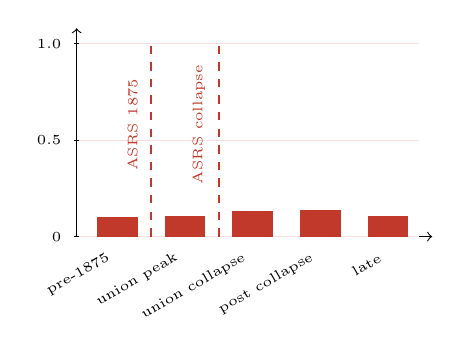
\begin{tikzpicture}[x=0.86cm,y=2.45cm]
  \draw[->] (0,0) -- (5.25,0);
  \draw[->] (0,0) -- (0,1.08);
  \foreach \y/\label in {0/0,0.5/0.5,1.0/1.0} {
    \draw[DismissalRed!15] (0,\y) -- (5.05,\y);
    \draw (-0.04,\y) -- (0.04,\y) node[left=3pt] {\tiny \label};
  }
  \fill[DismissalRed] (0.30,0) rectangle (0.90,0.100);
  \fill[DismissalRed] (1.30,0) rectangle (1.90,0.108);
  \fill[DismissalRed] (2.30,0) rectangle (2.90,0.130);
  \fill[DismissalRed] (3.30,0) rectangle (3.90,0.138);
  \fill[DismissalRed] (4.30,0) rectangle (4.90,0.108);
  \draw[dashed,thick,DismissalRed] (1.10,0) -- (1.10,1.02);
  \node[rotate=90,anchor=south,DismissalRed] at (1.04,0.58) {\tiny ASRS 1875};
  \draw[dashed,thick,DismissalRed] (2.10,0) -- (2.10,1.02);
  \node[rotate=90,anchor=south,DismissalRed] at (2.04,0.58) {\tiny ASRS collapse};
  \node[below,rotate=30,anchor=east] at (0.60,-0.08) {\tiny pre-1875};
  \node[below,rotate=30,anchor=east] at (1.60,-0.08) {\tiny union peak};
  \node[below,rotate=30,anchor=east] at (2.60,-0.08) {\tiny union collapse};
  \node[below,rotate=30,anchor=east] at (3.60,-0.08) {\tiny post collapse};
  \node[below,rotate=30,anchor=east] at (4.60,-0.08) {\tiny late};
\end{tikzpicture}
\end{minipage}

\vspace{0.18cm}
\scriptsize
\textbf{Promotion rate:} Share of workers who attained Goods Guard or Shunter grade within the observation window. LNWR Birmingham Guards register only ($n=423$ after cleaning).\\
\textbf{Dismissal rate:} Share of workers whose remarks column contains keywords: \textit{dismiss, discharg, resign, left service, removed}. Includes voluntary and involuntary exits; cannot distinguish between them.
\end{frame}

\begin{frame}{Ruling Out Composition Effects}
\begin{columns}[T,onlytextwidth]
\column{0.48\textwidth}
\textbf{\color{RailwayBlue}Full Sample}
\vspace{0.15cm}

\small
\begin{tabular}{lrr}
\toprule
\textbf{Period} & \textbf{Rate} & \textbf{N} \\
\midrule
pre-1875 & 0.500 & 10 \\
union\_peak & 0.486 & 37 \\
union\_collapse & 0.609 & 23 \\
post\_collapse & 0.738 & 65 \\
late & 0.726 & 288 \\
\bottomrule
\end{tabular}

\column{0.48\textwidth}
\textbf{\color{RailwayBlue}Excl. Engine Drivers \& Firemen}
\vspace{0.15cm}

\small
\begin{tabular}{lrr}
\toprule
\textbf{Period} & \textbf{Rate} & \textbf{N} \\
\midrule
pre-1875 & 0.500 & 6 \\
union\_peak & 0.472 & 36 \\
union\_collapse & 0.722 & 18 \\
post\_collapse & 0.789 & 57 \\
late & 0.774 & 226 \\
\bottomrule
\end{tabular}
\end{columns}

\vspace{0.5cm}
\footnotesize The post-1880 recovery is not driven by engine drivers and firemen, the grades most directly affected by ASLEF's 1880 split.
\end{frame}

\end{document}
